
%(BEGIN_QUESTION)
% Copyright 2011, Tony R. Kuphaldt, released under the Creative Commons Attribution License (v 1.0)
% This means you may do almost anything with this work of mine, so long as you give me proper credit

This level-control system does not appear to be regulating vessel liquid level correctly.  The SP is set for 2.5 feet (out of a 0-5 foot range), but the PV display on the controller faceplate registers 3.74 feet.  You happen to notice that the controller output reads 100\% on the faceplate:

$$\includegraphics[width=15.5cm]{i00337x01.eps}$$

A field operator informs you that a sightglass on this vessel reads 3 feet 9 inches, and the control valve stem position is approximately 40\% open.

\vskip 10pt

Identify the likelihood of each specified fault for this control system.  Consider each fault one at a time (i.e. no coincidental faults), determining whether or not each fault could independently account for {\it all} measurements and symptoms in this circuit.

% No blank lines allowed between lines of an \halign structure!
% I use comments (%) instead, so that TeX doesn't choke.

$$\vbox{\offinterlineskip
\halign{\strut
\vrule \quad\hfil # \ \hfil & 
\vrule \quad\hfil # \ \hfil & 
\vrule \quad\hfil # \ \hfil \vrule \cr
\noalign{\hrule}
%
% First row
{\bf Fault} & {\bf Possible} & {\bf Impossible} \cr
%
\noalign{\hrule}
%
% Another row
LT out of calibration (outputting wrong current) &  &  \cr
%
\noalign{\hrule}
%
% Another row
LIC input out of calibration (not interpreting signal properly) &  &  \cr
%
\noalign{\hrule}
%
% Another row
LIC output out of calibration (not sending correct mA signal to I/P) &  &  \cr
%
\noalign{\hrule}
%
% Another row
I/P out of calibration (not outputting correct pressure) &  &  \cr
%
\noalign{\hrule}
%
% Another row
Control valve is oversized &  &  \cr
%
\noalign{\hrule}
%
% Another row
Control valve is undersized &  &  \cr
%
\noalign{\hrule}
%
% Another row
LIC is poorly tuned (not making good control ``decisions'') &  &  \cr
%
\noalign{\hrule}
%
% Another row
Instrument air supply not at full pressure &  &  \cr
%
\noalign{\hrule}
} % End of \halign 
}$$ % End of \vbox

Also, explain how the principle of {\it correspondence} may be used to determine which portion of this control system (measurement, controller, output) the problem is located in.

\vfil 

\underbar{file i00337}
\eject
%(END_QUESTION)





%(BEGIN_ANSWER)

This is a graded question -- no answers or hints given!

%(END_ANSWER)





%(BEGIN_NOTES)

The controller's PV indication corresponds with the sightglass, which means the input (measurement) portion of this system works like it should.  The controller's output indication, however, does {\it not} correspond with the observed valve stem position, indicating a problem within that portion of the system.

% No blank lines allowed between lines of an \halign structure!
% I use comments (%) instead, so that TeX doesn't choke.

$$\vbox{\offinterlineskip
\halign{\strut
\vrule \quad\hfil # \ \hfil & 
\vrule \quad\hfil # \ \hfil & 
\vrule \quad\hfil # \ \hfil \vrule \cr
\noalign{\hrule}
%
% First row
{\bf Fault} & {\bf Possible} & {\bf Impossible} \cr
%
\noalign{\hrule}
%
% Another row
LT out of calibration (outputting wrong current) &  & $\surd$ \cr
%
\noalign{\hrule}
%
% Another row
LIC input out of calibration (not interpreting signal properly) &  & $\surd$ \cr
%
\noalign{\hrule}
%
% Another row
LIC output out of calibration (not sending correct mA signal to I/P) & $\surd$ &  \cr
%
\noalign{\hrule}
%
% Another row
I/P out of calibration (not outputting correct pressure) & $\surd$ &  \cr
%
\noalign{\hrule}
%
% Another row
Control valve is oversized &  & $\surd$ \cr
%
\noalign{\hrule}
%
% Another row
Control valve is undersized &  & $\surd$ \cr
%
\noalign{\hrule}
%
% Another row
LIC is poorly tuned (not making good control ``decisions'') &  & $\surd$ \cr
%
\noalign{\hrule}
%
% Another row
Instrument air supply not at full pressure & $\surd$ &  \cr
%
\noalign{\hrule}
} % End of \halign 
}$$ % End of \vbox

%INDEX% Basics, control loop troubleshooting: isolating area of fault by correspondence

%(END_NOTES)


